\section{Semi-Supervised Learning}
\label{sec:semisupervised}
While it makes sense to treat searches for new physics or rare signatures as a supervised classification problem, an alternative approach is to let an algorithm learn intrinsic features from an unlabeled dataset and then evaluate whether this self-learned information can be used to separate signal from background processes. This type of approach is called semi-supervised learning because an algorithm identifies patterns in the data in an un-supervised way and is then evaluated using known classification information.

\subsection{Clustering}
\label{sec:clusters}
k-means. Other? PCA?


\subsection{Auto-encoders}
\label{sec:AE}

An autoencoder (AE) is an unsupervised machine learning architecture used for detecting anomalies that differ significantly from the data used to train the network. The structure of the AE compresses the input information into a lower-dimensional representation called the latent space. This compression `encodes' the most important features of the training data into the latent space, while the second half of the network `decodes' the latent space back into a representation approaching the original inputs.

This construction fundamentally changes the meaning of the loss calculation-- rather than computing the loss between a prediction and a target, the AE loss is a measure of how well the network reproduces the original inputs after encoding and decoding. Inputs that differ significantly from the data used to train the AE will not be properly reconstructed, and anomalies can be identified by selecting events with large losses. Training with Monte Carlo simulations allows for a semi-supervised cross-check on AE performance since the classes of training and testing samples are known in advance.

Because AE anomaly detection relies on a well-modeled understanding of background processes, the network was trained using only QCD events. Additional models were trained by substituting the pure-QCD training sample with training samples consisting of mixtures of QCD and di-Higgs events to test the stability of the method against signal contamination. No significant deterioration was observed for reasonable levels of contamination. The AE used for di-Higgs detection was built using the Keras package~\cite{chollet2015keras} and consists of an input layer, a single hidden layer, and an output layer. Eleven reconstructed variables were selected for use in the AE. 

\begin{figure}[!h] 
\begin{center}
\includegraphics*[width=0.75\textwidth] {AE/figures/ae_PCA_11vars}
\caption{PCA performed on the selected eleven kinematic inputs. The x-axis indicates the number of PCA features, and the y-axis indicates the variance. Choosing the optimal size for the latent space requires identifying the point of diminishing variance return.}
  \label{fig:ae_pca}
\end{center}
\end{figure}

The output layer is a mirror of the input layer and therefore has 11 nodes. A PCA analysis (shown in Figure~\ref{fig:ae_pca}) was used to determine that a latent space of three nodes was optimal. The hidden layer and output layer use ReLU and sigmoid activation functions respectively. An L2 regularization term was added to the hidden layer to avoid over-fitting. %Afterwards the model was compiled using the ‘adam’ optimizer with the mean-squared error loss. Finally, the model was fit on the training data along with the validation data for 10000 epochs. The ‘EarlyStopping’ function was used to shorten training time by stopping training after the validation accuracy didn’t increase by 0.001 for 50 epochs. The batch size during training was set to 1024 in order to both decrease training time and prevent overfitting.
Because training an autoencoder is an unsupervised and unlabeled process, there is no prediction of whether a given event is signal or background. Since di-Higgs events should be relatively anomalous compared to the QCD training set, signal events should have a relatively larger average loss value. Cutting on the loss function allows for a significance to be calculated for comparison with other methods.

\begin{figure}[!h] 
  \begin{center}
    \subfloat[]{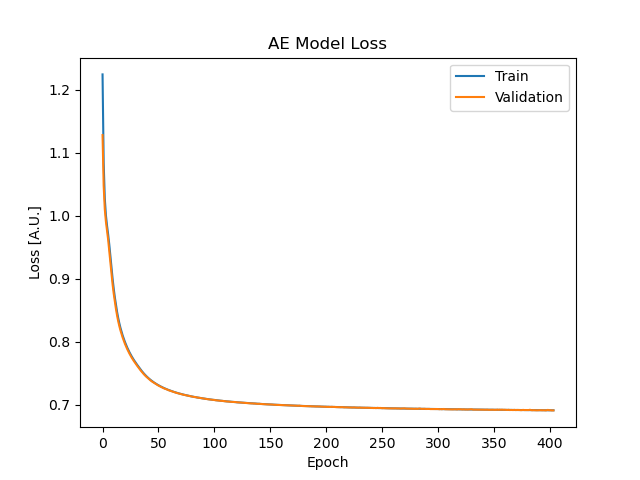
\includegraphics[width = 3in]{AE/figures/ae_modelLoss_qcdTrain_v2}} 
    \subfloat[]{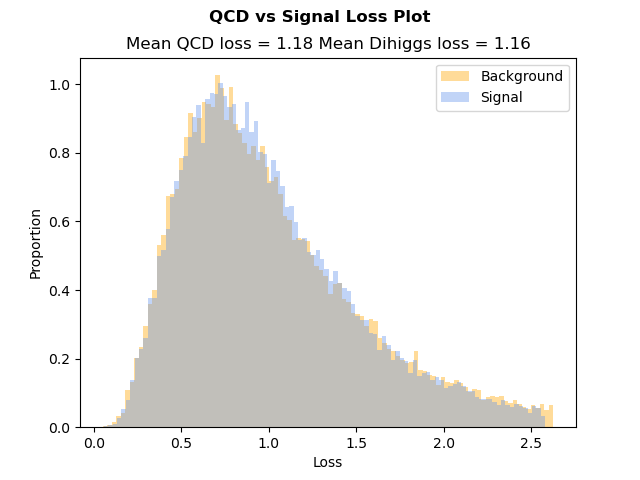
\includegraphics[width = 3in]{AE/figures/ae_finalLossDistribution_qcdTrain_v2}}\\
    \caption{(Left) The loss of the AE during QCD training/reconstruction converged after 700 epochs. (Right) The loss distribution generated by the AE when being tested on QCD and di-Higgs event data separately.}    
  \label{fig:ae_trainPredLoss}
\end{center}
\end{figure}

Training for several hundred epochs leads the model to converge, and it reaches an asymptotic loss value near 0.7 (see Figure~\ref{fig:ae_trainPredLoss}). Requiring the loss to be larger than 0.05 yields a best significance of $\sigma$ = 0.81$\pm$0.01. This significance value may be somewhat misleading since the signal and background loss distributions have little separation. The highest significance result effectively is a cut that keeps nearly all events. This suggests that the kinematic inputs used in training do not significantly differ between signal and background processes after the latent space compression.

%\begin{figure}[!h] 
%\begin{center}
%\includegraphics*[width=0.75\textwidth] {AE/figures/ae_finalSignalPredictions_qcdTrain}
%\caption{Signal predictions made by the AE based on the loss distributions from Fig. 3. The $S/\sqrt{B}$ best cut was placed near 0.1, indicating that the AE was not able to sufficiently distinguish di-Higgs da%ta from QCD data.}
%  \label{fig:ae_signalPred}
%\end{center}
%\end{figure}

